% !TEX TS-program = xelatex
% !TEX encoding = UTF-8 Unicode

% GSET Summer 2023 - Tennessee Technological University
% Tristan Hill - June 07, 2023
% Turtorial 4 - List Methods - Shopping List

\documentclass[12pt]{article}

% Custom Preamble
%\usepackage{/home/thill/Documents/lectures/cpp_workshop/modules/cpp_tutorial} 
\usepackage{/mnt/c/Users/thill/Documents/courses/py_workshop/modules/py_tutorials}


% Title and Misc
\newcommand{\MNUM}{4} %Module Number
\newcommand{\MNAME}{Lists} %Module Name
\newcommand{\TNAME}{Shopping List} %Tutorial Name
\pagestyle{myheadings}
\markright{{\large GSET - Introduction to Programming with Python}}

\begin{document}

\thispagestyle{plain}

\begin{center}
   {\bf \large GSET - Introduction to Programming with Python - Summer 2023} \vspace{5mm}\\
   {\bf \Large \MNAME \hspc -  Tutorial\hspc\MNUM\hspc - \TNAME}\vspace{3mm}\\
   
\end{center}

%\hspace*{3cm}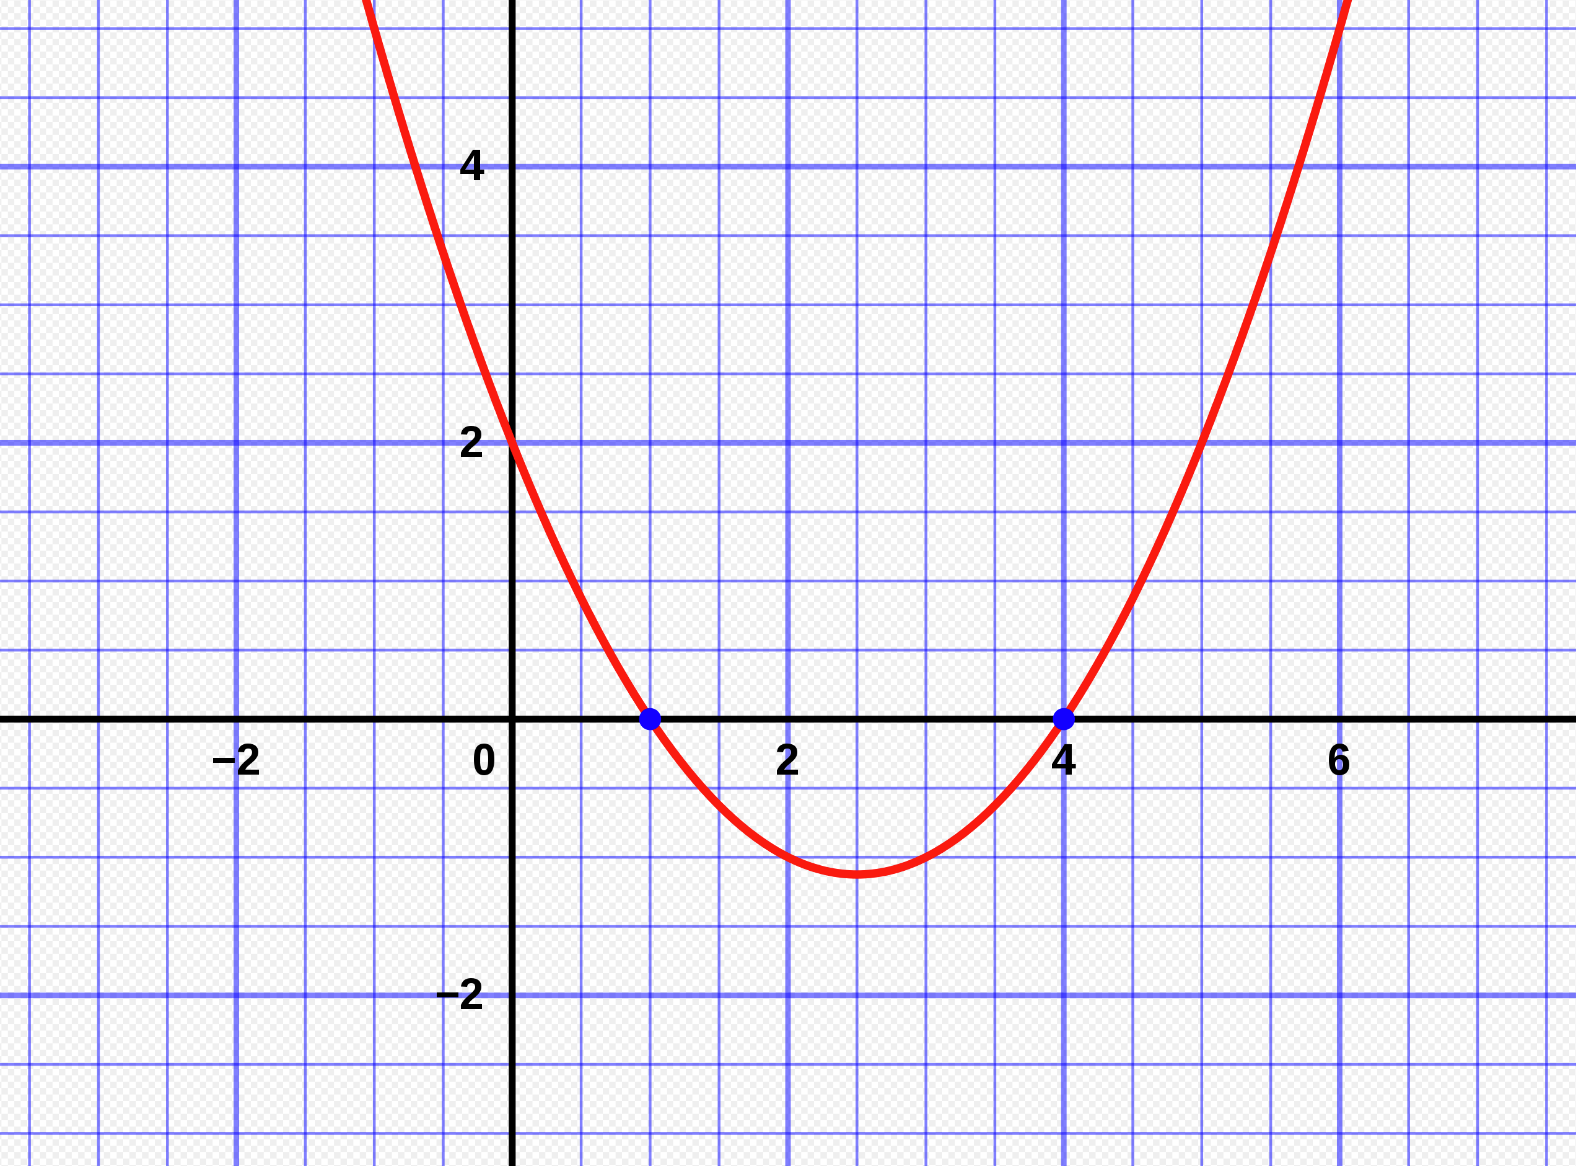
\includegraphics[scale=.15]{quad_equ.png} 

\begin{description}[labelindent=1cm]
	
			\item [\textbf{ \Large Overview}] \textbf{ \Large :}\\
			You will practice using lists in a Python program. The {\it print} function will be used to display formatted strings to the command window, and the input function will be used to get information from the user during program execution. \\
 	
	\item[\textbf{\underline{System Requirements:}}] \hfill \vspace{0mm}

\begin{itemize}
	\item {\bf Computer}: A computer is required to complete this tutorial. Any OS should work.
	\item {\bf Python:} You can use the online Python compiler ( \href{https://www.online-python.com/online_python_compiler}{Online Python Compiler}  ) or a Python system of your choice.
\end{itemize}

	\item[\textbf{\underline{Background:}}] \hfill \vspace{0mm}
	
	\begin{description}

	 	\item [\textbf{Shopping List }] \textbf{ \Large :}\\   
            You are going to write a program to manage a shopping list. Your list can be for used for anything (e.g. groceries, a cool robot). This list will contain all the items you intend to purchase and their predicted prices.
            
      
   \item[\textbf{\underline{Problem Statement:}}] \hfill \vspace{0mm}

	\begin{itemize}

		\item Given: Desired items to purchase and predicted prices
		
		\item Complete: Generate a program to define, edit, and display the items and prices of item in the list
	\end{itemize}      


	\end{description}


\newpage
\item[\textbf{\underline{Program Minimum Requirements:}}] \hfill \vspace{0mm}

The program should accomplish the following tasks. 

\begin{enumerate}
	
	\item Part 1 
		\begin{enumerate}
	      \item
	      Initialize a list named \lstinline{items} containing at the names of least 5 things to be purchased. Store the names of the items in the list as strings.  \\
	      \item
	      Initialize a second list named \lstinline{prices} containing the prices of the items to be purchased. The order of the prices should match the order of the list of items.   	
	      \item
	      Print the initial list of items and the list of prices in a readable format.  
		\end{enumerate}	 

	\item Part 2
		\begin{enumerate}
	      \item
	     	Use the \lstinline{input} function to get a new item from the user to add to the list. Append the item to the end of the list and update the prices list appropriately. 
	      \item
	      Use the \lstinline{input} function to get a second new item from the user to add to the list. Insert the item near the middle of the list and update the prices list appropriately. 
	      \item 
	      Print the modified list of items and the list of prices in a readable format.  
		\end{enumerate}	

	\item Part 3
	\begin{enumerate}
      \item Display the most expensive item in the list and the corresponding price.
      \item Display the least expensive item in the list and the corresponding price.
      \item Display the combined price of all the items in the list and the average price of items in the list.
      \item Remove the most expensive item from the list and the corresponding price from the prices list.
      \item Display the combined price of all the items in the list and the average price of items in the list after removing the most expensive item.
	\end{enumerate}


	\item Optional Advanced Features:
		\begin{itemize}
			 
			\item Modify the program show the list of items from most expensive to least expensive
			\item Modify the program show the list of items in alphabetical order
			\item Create a second version of the program that uses a dictionary instead of two lists
			\item Give the user the option to remove or not remove items
		    
		\end{itemize}	

	\end{enumerate}
\newpage

\item[\textbf{\underline{Example Code:}}] \hfill \vspace{0mm}

	%\begin{minted}{cpp}
	\begin{lstlisting}

# Lists - GSET - Summer 2023 
	

	
	\end{lstlisting}
	%\end{minted}
		


	\item[\textbf{\underline{Part 3 - Testing:}}] \hfill \vspace{0mm}
	\begin{enumerate}
	
		\item Complete the Python code to the solve the problem described. \\\\
		
		\item Test your code with different inputs. Is the answer correct? How do you know? Are there certain inputs that do not work? \\\\
		
		\item Save your code with the download button or use copy and paste. You can view and edit the code in any text editor. Also, save a copy of the program output for your tutorial summary. \\\\

	\end{enumerate}

\newpage
\item[\textbf{\underline{Solution Code:}}] \hfill \vspace{0mm}

\begin{lstlisting}

COMING SOON
	
\end{lstlisting}

\item[\textbf{\underline{Tutorial Summary:}}] \hfill \vspace{3mm}\\ 
Write a brief summary of what you accomplished and what you struggled with the most. 

Include the following items in the summary:
\begin{itemize}

\item a copy of the output of your program
\item a description of what the program does and how to use it

\end{itemize}


\item[\textbf{\underline{Submission on Teams:}}] \hfill \vspace{3mm}\\ 
Use the appropriate assignment folder on ilearn to submit your program and summary. Submit the following items with your TNTech username in the filenames as shown below. \vspace{0mm}\\

\underline{Files for Tutorial 4 (TNTech Username : twhill21)}

\begin{itemize}

\item Tutorial Summary: \textbf{ twhill21\_summary4.txt}

\item Python Source Code: \textbf{ twhill21\_tutorial4.py}

\end{itemize}


\item[\textbf{\underline{Tutorial Complete:}}] \hfill \vspace{3mm}\\ 
	Congratulations, after completing {\it Tutorial 4 - The Shopping List}, you have begun learning to program in Python! You are now ready to start learning about more complex data structures and program flow. \\

\end{description}
\end{document}

